\documentclass[12pt]{article}
\usepackage{amsmath}
\usepackage{amssymb}
\usepackage{listings}
\usepackage{graphicx}
\usepackage{nopageno}
\usepackage{paralist}
\usepackage{sparklines}
\usepackage{tabularx}
\usepackage{booktabs}
\usepackage{color}

\definecolor{listingbg}{rgb}{0.99, 0.96, 1}
\definecolor{commentbg}{rgb}{0.3, 0.3, 0.8}
\lstloadlanguages{Haskell}
\lstnewenvironment{code}
    {\lstset{}%
      \csname lst@SetFirstLabel\endcsname}
    {\csname lst@SaveFirstLabel\endcsname}
    \lstset{
      language=Haskell,
      basicstyle=\footnotesize,
      flexiblecolumns=false,
      basewidth={0.5em,0.45em},
      sensitive=true,
      numberstyle=\tiny,
      numberblanklines=true,
      literate={+}{{$+$}}1 {/}{{$/$}}1 {*}{{$*$}}1 {=}{{$=$}}1
               {>}{{$>$}}1 {<}{{$<$}}1 {\\}{{$\lambda$}}1
               {\\\\}{{\char`\\\char`\\}}1
               {->}{{$\rightarrow$}}2 {>=}{{$\geq$}}2 {<-}{{$\leftarrow$}}2
               {<=}{{$\leq$}}2 {=>}{{$\Rightarrow$}}2 
               {\ .}{{$\circ$}}2 {\ .\ }{{$\circ$}}2
               {>>}{{>>}}2 {>>=}{{>>=}}2
               {|}{{$\mid$}}1               
    }

\DeclareMathOperator*{\argmax}{arg\,max}
\DeclareMathOperator*{\Merge}{Merge}
\DeclareMathOperator*{\Range}{Range}

\renewcommand{\Pr}[1]{\ensuremath{\mathrm{Pr}\{ #1 \}}}

\begin{document}
\frenchspacing

\author{Joseph Abrahamson}
\title{520.666: Project \#3}

\maketitle

\section{Agglomerative letter clustering}
\label{sec:agg}

One kind of entropy-justified tree can be grown from the bottom up by
merging sets of objects such that each merge is between the two sets
with the largest mutual information. If you have a set of elements
$\mathcal{A} \triangleq \{a_i\}_{i = 0}^N$, then you can begin with
$\mathcal{S}_0 \triangleq \{s_i = \{a\} : a \in \mathcal{A}\}$ and
perform the merge $\Merge_{0 \to 1}(i, j) \implies \mathcal{S}_1 =
\Merge_{0 \to 1}(i, j)(\mathcal{S}_0) = \mathcal{S}_0\backslash\{s_i,
s_j\} \cup \{(s_i \cup s_j)\}$. We then define the algorithm as the
sequential application of the $(N-1)$ merges $$\Merge_{0\to1},
\Merge_{1\to2}, ... \Merge_{(N-1)\to N}$$ such that each merge
satisfies
\begin{align}
  \Merge_{k\to(k+1)}(i, j) : (s_i, s_j) = \argmax_{\Merge(i, j) : s_i, s_j \in \mathcal{S}_k}
    I(\Merge(i, j)(\mathcal{S}_k))
\end{align}
where
\begin{align}
  I(\mathcal{S}_k) &\triangleq \sum_{l, m : s_l, s_m \in \mathcal{S}_k} f(s_l,
  s_m) \log\frac{f(s_l, s_m)}{f(s_l) f(s_m)} \\
  f(s) &\triangleq \sum_{a \in s} f(a) \\
  f(s_l, s_m) &\triangleq \sum_{a_l \in s_l} \sum_{a_m \in s_m} f(a_l, a_m)
\end{align}
and the unigram and bigram frequencies are defined on the original
atomic set $f(a) = f(\langle a \rangle)$ and $f(a_i, a_j) = f(\langle
a_i a_j\rangle)$. Note that since each merge operation reduces the
number of sets in $\mathcal{S}_k$ by 1, $|\mathcal{S}_k| = N-k$,
$\mathcal{S}_{(N-1)} = \{\mathcal{A}\}$ providing a
simple count for how many operations need to be performed.

This recursive pairing behavior leads naturally the construction of a
tree with the atoms in $\mathcal{A}$ at the leaves and also implies
that if you split the full tree into two haves starting at the root
node then the two sets containing the atoms from the left and right
halves will have a small mutual information $I$ value, though it is
not clear that it is the smallest possible split.

\subsection{Experimental results}

Performing this sort of agglomerative clustering over a set of atoms
defined as the 26 English letters plus space \texttt{' '} formed an
agglomerative tree (displayed in Figure
\ref{fig:agglomerative-bubbles}). This tree demonstrates similar
entropic properties of English letters as an HMM model of English text
in that the first-grouping (derived by splitting the tree at the root
node) separates the atoms into the set of ``vowels $+$ space'' and
``consonants'' which corresponds to the two-state HMM model's emission
densities. The second-grouping (derived by performing a first-grouping
on each of the above sets) produces the 4 sets (\texttt{'aoiue'},
\texttt{' '}, \texttt{'rxlnsydg'}, \texttt{'vzkmfjqbpcwth'}) which
clearly splits the space from the vowels and splits consonants into
two groups. This corresponds in part to the 4-state HMM model's
emission densities, although the consonant breakdown was different.

\begin{figure}
  \centering
  \makebox[\textwidth]{\includegraphics[width=7in]{agglomerative-bubbles}}
  \caption{\textbf{Agglomerative clustering of English letters on a
      training text leads to this letter grouping tree.} Grey circles
    are drawn such that at any particular level in the hierarchy,
    atoms contained within the circle are clustered together. Thus,
    smaller circles imply groupings closer to the leaves (with the
    leaves displayed in white) and larger circles are sets closer the
    the root of the tree.}
\label{fig:agglomerative-bubbles}
\end{figure}

\section{Bitstring encoded decision trees}

Using the bottom-up method of agglomerative clustering from section
\ref{sec:agg} we can generate a string of binary predictors of any
atom $a \in \mathcal{A}$ from the path between the root node and that
particular atom. Such bitstrings can be encoded such as
$\langle$LLRLRRLRR$\rangle$ and unambiguously select a particular
atom. Moreover, any left substring of a predictor of this form will
denote the subset of $\mathcal{A}$ that both contains $a$ and has the
maximual mutual information with $a$. In this way we can guarantee
that if an actor interested in predicting $a$ knew some left substring
of $a$'s bitstring encoding, the best next question for that actor to
ask would be the leftmost unseen ``bit'' in the string.

This leads directly to a sensible algorithm for decision tree growth
by suggesting a choice of best possible questions at each node. In
particular, for a model with $n$ predictors, moving through the
decision tree should be an exercise of walking down the paths in the
agglomerative tree leading to each of the $n$ predictors
independently, one question at a time. At any node in the decision
tree, you pick one of $n$ questions depending on which predictor will
provide the most information about the predicted quantity when we
learn one more bit about it.

So with that set of admissible questions, we greedily build a decision
tree, recursively picking the best possible question of the $n$
admissible ones by measure of the lowest post-split entropy on the
predictor. This means that if in a particular node we have limited the
admissible conditionals to a set $M$, and after asking a question $q$
this is split into the disjoint sets $M_{q^+}$ and $M_{q^-}$, we
search for the $q$ such that
\begin{align}
  \arg\min_q \left\{ \frac{|M_{q^+}|}{|M|}H(x | x \in M_{q^+}) +
  \frac{|M_{q^-}|}{|M|}H(x | x \in M_{q^-})\right\} \label{node-entropy}
\end{align}

Note that different from the algorithm advised, here we choose $q$
conditional only locally to the node we're considering splitting. This
is because the $q$ which is the minimizer of \eqref{node-entropy} will
be that maximizer invariant of the state of the rest of the tree and
thus we do not need to compute the global entropy given each possible
$q$, just the local entropy.

The stopping criterion for this tree involves the computation of the
same entropy measures on a held-out set of data. So long as the
entropy change induced by a split is greater in magnitude than a
certain cutoff (0.005 bits in this case), the split induced by entropy
minimizer question $q$ is accepted as a new branching node in the
decision tree. If the held out entropy change is not larger than that
cutoff, however, that node is barred from splitting further.

By structuring the tree growth algorithm like this (most importantly
noting the locality of the $q$ minimizer condition) an elegant
recursive algorithm can be performed (Haskell pseudocode)

\begin{code}
buildDTree :: ([Obs], [Obs]) -> (Double, Double) -> QList -> DTree Question ()
buildDTree (dev, ho) (h_dev, h_ho) qlist = 
  if h_ho - h_ho' > reductionThreshold
  then Branch bestQ (buildDTree (dev_left, ho_left) (h_dev', h_ho') qlst')
                    (buildDTree (dev_right, ho_right) (h_dev', h_ho') qlst')
  else Leaf ()
  where
    h_ho'  = splitEntropy ho bestQ
    h_dev' = splitEntropy dev bestQ
    (dev_left, dev_right) = splitByQuestion dev bestQ
    (ho_left, ho_right) = splitByQuestion ho bestQ
    (bestQ, qlist') = minimumBy (comparing (splitEntropy dev)) qlist
\end{code}

where each node either generates a new branch or terminates and the
children of the new branches are recursively generated by the same
procedure.

\subsection{Concerns with smoothing}

Since the leaf node frequencies are often very specific, it is very
possible for unseen data to have a zero observed frequency at the node
it is sorted into. Since this would render the entire event as
impossible, smoothing is necessary.

The suggested linear smoothing method, proposed in Jelinek [1997], is
flawed in that in practice it ties smoothing weights in such a way
that some leaf distributions become unnormalized. This occurs because
the path lengths through the trees are not guaranteed to be identical
and such leanred parameters tied to tree depth will only sum to 1 for
maximally long paths in the tree.

To remedy this, one can use an adaptive smoothing method which
generates smoothing parameters conditional on the path through the
tree. For convenience and coherance across the tree, we demand that
each adaptive process returns similar results for any path, and for
purposes of training we demand that it has some kind of global
parametrization which does not depend on the path. This constraints
together suggest that the parameters of each adaptive process can be
tied and trained simultaneously.

In short, we are looking for a function $\lambda_n(N,
\mathbf{\Theta})$ for $n \le N$, $N$ being the length of the
particular path, and $|\mathbf{\Theta}| \le N_{min}$, $N_{min}$ being
the length of the shortest path in the tree. Additionally, $\forall N,
\sum_i^N \lambda_i(N, \mathbf{\Theta}) = 1$ in order to ensure
normalization.

One particular choice satisfying these constraints is the
Beta-Binomial distribution
\begin{align}
  \lambda_n(N, \alpha, \beta) 
  &= {N \choose n} \frac{B(\alpha + n, \beta + (N-n))}{B(\alpha, \beta)} \\
  B(\alpha, \beta) 
  &\triangleq \frac{\Gamma(\alpha)\Gamma(\beta)}{\Gamma(\alpha + \beta)}
\end{align}

with $\Gamma(x) \triangleq \int_0^\infty t^{x-1} e^{-t} dt$ being the
Gamma function extension of factorial. While this choice of weight
distribution is completely arbitrary, it does cover any interpolation
which can be described entirely by unbounded weighting of the unigram
and leaf node models along each path. Included in this set is any
``monomodal'' interpolation for which a certain range along the path
is favored along with the ``tail-weighted'' interpolation where only
the unigram and leaf-node models are considered and they are weighted
equally (see Figure \ref{fig:betabinomial}).

\begin{figure}
  \centering
  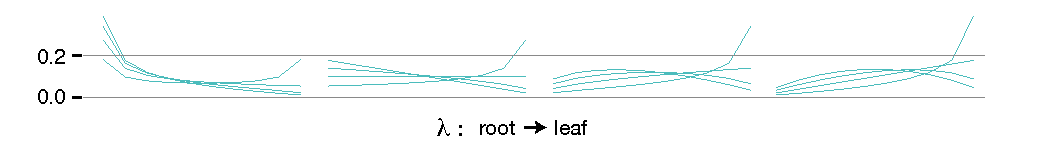
\includegraphics[width=\linewidth]{betabinom}
  \caption{\textbf{Beta-binomial distributions for various choices of
      parameters $(\alpha, \beta)$.}}
  \label{fig:betabinomial}
\end{figure}

This method of smoothing has the distinct disadvantage of having no
clear Baum algorithm update method (though one may be possible to
derive). Instead, since the entire family of adaptive methods is
parameterized by exactly two free parameters, both varying on $(0,
\infty)$, we can make the reparameterization $(\alpha^\star,
\beta^\star) = \left(\sqrt{\frac{1}{1+\alpha}},
  \sqrt{\frac{1}{1+\beta}}\right)$ and do a constrained grid search
within $(0,1)^2$ then pick the values which maximize likelihood over a
held out data set.

\subsection{Experimental results}

Using the same training text that, in whole, generated the
agglomerative tree over English letters, to generate a 4-gram
prediction task of English spelling, a decision tree was generated
according to the above algorithm. This involved searching through a
list of 3 questions at each potential branching decision, one for each
history letter. The final tree has 125 fully-specified ``leaf''
distributions corresponding to a complete partitioning of the trigram
histories into 125 fine-grained equivalence classes.

Various representations of the questions asked in the tree are shown
in Figures \ref{fig:bs_wedges} and \ref{fig:bs_examplepaths}. In
particular, from Figure \ref{fig:bs_wedges} it is clear that the
algorithm tends to clarify the most recent character, $w_3$, out to
often 4 or 5 questions before alternating between $w_1$ and $w_2$.

Figure \ref{fig:bs_examplepaths} gives concrete examples of many
paths, demonstrating a range of the length of time spent clarifying
the most recent letter before beginning to alternate between $w_1$ and
$w_2$.

% Figure \ref{fig:bs_jumpcounts} is a transition frequency matrix
% between various questions and demonstrates with its strong 1st
% superdiagonal that once a character is queried, it tends to be further
% clarified (especially $w3$, the word directly preceeding the predicted
% character).

While the decition tree here was trained on a text of 25k characters,
with a 5k letter smoothing verification text, and a 5k test text
retained. Model perplexity was measured at 8.31 on this test text
which represents an improvement of 8.73 over the unigram
model. Surprisingly, the optimizing smoothing distribution
coefficients were $\alpha \approx 10^{4}$, $\beta \approx 10^{-4}$ which places
nearly all of the weight on leaf node distributions. This held true
for if the test data set was used to evaluate the smoothing parameters
as well, suggesting that, at least for the data sets used here, the
leaf distributions were far better than any parent branch
distributions and that the unseen 4-gram problem was not problematic
so long as the probability assigned was non-zero.


\begin{figure}
  \centering
  \vspace{-1in}
  \makebox[\textwidth]{\includegraphics[width=7in]{bs_wedges}}
  \caption{\textbf{A representation of the bitstring question grown
      decision tree for English spelling.} Here the root node is
    represented as the circle in the center with each label $x:y$
    meaning that the predictive question asked at that node was of the
    $y$th most informative bit of the $x$th word (with strings labeled
    $\langle w_1 w_2 w_3 w_4 \rangle$ and $w_4$ being
    predicted). Additionally, each node's wedge is colored to
    correspond with the word being queried.}
  \label{fig:bs_wedges}
\end{figure}

\begin{figure}
  \centering
  \vspace{-1in}
  \makebox[\textwidth]{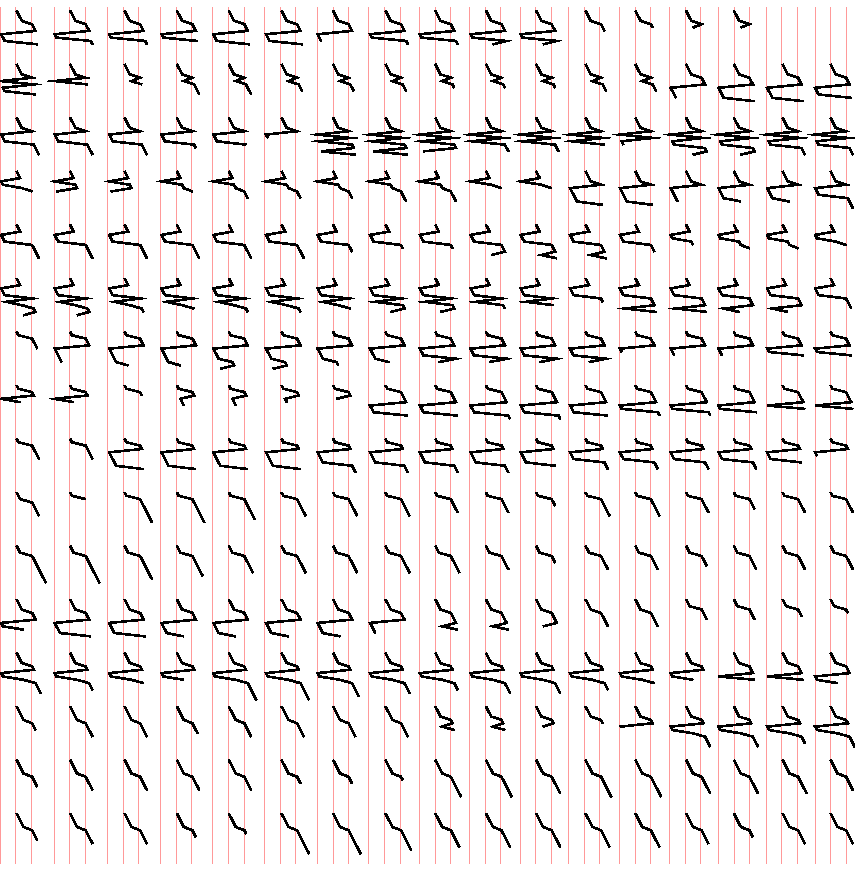
\includegraphics[width=7in]{bs_path_270}}
  \caption{\textbf{All 125 ``question paths'' extracted from the
      experimental decision tree.} The $x$-axis in each small multiple
    plot corresponds to an index into the concatenated bitstring
    $\langle b_1 b_2 b_3 \rangle$ where $b_i$ is the bitstring
    corresponding to $w_i$ in the observed 4-gram $\langle w_1 w_2 w_3
    w_4 \rangle$. The multiples are ordered from the leftmost path
    ($\langle$LLLLL $...\rangle$) in the lower left corner to the
    rightmost in the upper right and varies minimally from its
    horizontal neighbors. Each blue line then traces the questions
    asked on a random walk through the decision tree while the red
    lines denote character boundaries in the concatenated bitstring.}
  \label{fig:bs_examplepaths}
\end{figure}

% \begin{figure}
%   \centering
%   \makebox[\textwidth]{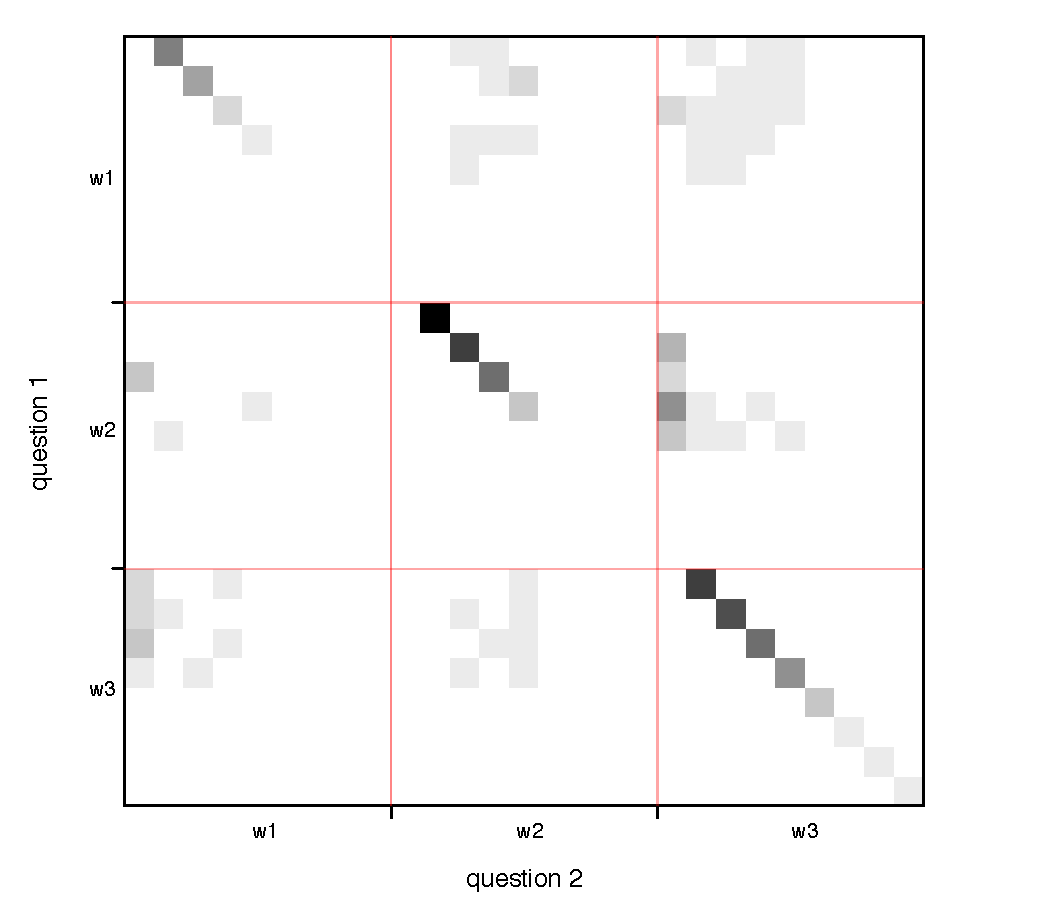
\includegraphics[width=4in]{bs_jumpcounts}}
%   \caption{\textbf{Question pair frequencies in the experimental
%       decision tree.} Here the $x$ and $y$ axes represent indices into
%     the concatenated predictive bitstring (see Figure
%     \ref{fig:bs_examplepaths}) and the colored bins represent pairs of
%     questions such that the $x$-axis question was asked after the
%     $y$-axis question and darker colors are more frequently observed
%     pairs across all paths in the decision tree.}
%   \label{fig:bs_jumpcounts}
% \end{figure}

\section{Using Chou-type questions}

While bitstring encoding of the alphabet is a logical way to
parameterize the space of permissible questions, that parameterization
reduces the space of questions greatly (after all, only 3 questions
are considered at any particular branch point). Chou's algorithm is a
way to parameterize a much larger space of questions while still
finding a greedy minimum.

The heart of Chou's algorithm is making allowable questions be of the
form ``$k(\mathbf{h}) \in \mathcal{A}$?'' where $k(\cdot)$ is some kind
of keying function, and $\mathcal{A}$ is a chosen subset of
$\Range(k)$. Thus, for a fixed $k(\cdot)$, selection questions in this
class involves finding the $\mathcal{A}$ which minimizes some cost
function (entropy, or, used here, the Gini Index).

Since this problem is still prohibitively large with
$2^{|\Range(k)-1|}$ options ($\sim 137$M for $\Range(k)$ being the
English alphabet) to search though, Chou's algorithm provides a method
of making a step $\mathcal{A}_{n} \to \mathcal{A}_{(n+1)}$ which
reduces the cost function and thus can be used iteratively to find a
locally optimal $\mathcal{A}$.

Of course, since the Chou algorithm only finds a locally optimal
$\mathcal{A}$, it's necessary to consider the sensitivity of the
algorithm to the bootstrapping $\mathcal{A}_0$ set.

Finally, with the Chou algorithm, there is the question of what to do
if a certain history is unseen but needs to be assigned to a
particular Chou optimizing step's $\mathcal{A}$. In this case, without
any data to suggest a solution, the algorithm described here takes a
``left default'' stance and moves those histories down the left
branch. If this occurs later during a likelihood evaluation, however,
it's also necessary to use distribution smoothing. The same smoothing
method as described for the bitstream encoded tree is used here.

\subsection{Experimental results}

A decision tree was formed by the Chou model using an identical
training and testing data set as the bitstring model. Considering the
abovementioned $\mathcal{A}_0$ sensitivity, three choices of
$\mathcal{A}_0$ were used \begin{inparaenum} 
\item the agglomerative model's first split: vowels and consontents
\item an uninformative split taking every other letter in alphabet
  order ($\mathcal{A}_0$ = \texttt{"acegikmoqsuwy "})
\item a maximum entropy choice found by searching once over all 137
  million choices of $\mathcal{A}_0$ (incidentally, $(\mathcal{A},
  \bar{\mathcal{A}}) = (\mathtt{"aeilnorst
    "},\texttt{"bcdfghjkmpquvwxyz"})$)
\end{inparaenum}. 

Smoothing parameters, also estimated using grid search over
$(\alpha^\star, \beta^\star)$, were identically optimized as the
bitstream tree again providing evidence that the leaf node
distributions do the best job of estimating the data even in spite of
impossible scenarios: just a small amount of probability weight put
into impossible events mitigates their effect.

Various parametric choices of the Chou-style decision tree and their
performance are summarized in Figure \ref{fig:stop-cutoff}. Of note,
the Chou-style trees tend to perform slightly ($< 1$ unit perplexity
improvement) better than similarly sized bitstream model
trees. Moreover, while the ``Alternating'' style $\mathcal{A}_0$
choice was rather arbitrary, it performs similarly to the maximal
entropy choice. Both of those, however, out perform the
vowel+consonant split $\mathcal{A}_0$ suggesting that such an informed
choice of $\mathcal{A}_0$ leads to an underexplored search space as
the Chou algorithm can quickly get stuck in local optima near that
solution.

\begin{figure}
  \centering
  \begin{tabularx}{\textwidth}{ lXXXX }
    & Unigram model & Vowel & Alternating & Maximum Entropy \\
    \toprule
    \textit{$5\times10^{-3}$ cutoff} & & & & \\
    \midrule
    \textit{Perplexity} & 17.05 & 10.55 & 8.06 & 8.36 \\
    \textit{Leaf count} & 1     & 100   & 302  & 248  \\
    \\
    \textit{$5\times10^{-4}$ cutoff} & & & & \\
    \midrule
    \textit{Perplexity} & 17.05 & 10.03 & 7.41 & 7.82 \\
    \textit{Leaf count} & 1     & 156   & 382  & 328  \\
    \bottomrule
  \end{tabularx}
  \caption{\textbf{Perplexity and leaf count for various Gini index
      cutoff values.} ``Cutoff'' denotes the cutoff value that the
    Gini index of the held-out data set must reduce by in order to
    accept a split. Unigram model is an unsplit root node decision
    tree, ``vowel'' represents initial $\mathcal{A}_0$ choices
    splitting the alphabet by vowels and consonants, ``Alternating''
    is the $\mathcal{A}_0$ choice such that letters are selected
    alternatingly in alphabetic order, and ``maximum entropy''
    represents the set choice $\mathcal{A}_0$ that maximizes entropy
    of the unigram distribution in the training text over all 137
    million possibilities.}
  \label{fig:stop-cutoff}
\end{figure}

The optimal Chou-style tree (cutoff = $5\times10^{-3}$,
``Alternating'' style $\mathcal{A}_0$) is pictured in Figure
\ref{fig:chou-tree} in a convention similar to Figure
\ref{fig:bs_wedges}. Of immediate note is that the strong tendency to
query the most recent letter in great detail before considering the
others has vanished. Instead, though the most recent letter dominates
the central branches of the tree, questions are arranged with greater
variety. 

\begin{figure}
  \centering
  \makebox[\textwidth]{\includegraphics[width=7in]{chou-tree}}
  \caption{\textbf{A depiction of the structure of an example
      Chou-style tree.} Branches of the decision tree radiate outward
    from the central root node (the circle). Colors and numbers
    represent which history item $\langle w_1 w_2 w_3 \rangle$ was
    used for the particular question in that tree branch. Specific
    sets used to determine each branch split are not depicted to
    reduce clutter.}
  \label{fig:chou-tree}
\end{figure}

\section{Conclusion}

In conclusion, tree based language models allow for very
computationally feasible language models which query increasingly
complex parameters of the history. In fact, both algorithms are able
to use greedy method to transform searches which have steps that are
exponential in history size to those merely polynomial.

While theoretically there is a great deal of difference between the
greedy methods that decide on the questions used in the decision tree,
within the limits of only using 4-gram history, it appears that both
the highly constrained bitstring method and the more general Chou
method perform roughly equivalently. 

The benefit comes from the ability to consider larger histories with
ease. For instance, increasing the Chou-style question model used here
to search for questions in 6-grams involves changing a single function
and reduces the model perplexity to 7.07 while less than doubling the
time to train and estimate. This would be clearly impossible using
more naive models of history equivalences.

\end{document}